\chapter{Uncertainty and Error Propagation}\label{chap:uncertainty}
Robots are systems that combine sensing, actuation, computation, and communication. All of its sub-systems are subject to a high degree
of uncertainty. This can be observed in daily life: phone calls often are of poor quality, making it hard to understand the other party,
characters are difficult to read from far away,  the front wheels of your car slip when accelerating on a rainy road from a red light,
your wireless device has a hard time getting a connection, or your neural network mistakes a cat for a dog. In robotics, measurements
taken by on-board sensors are sensitive to changing environmental conditions and subject to electrical and mechanical limitations.
Similarly, actuators are not accurate as joints and gears have backlash and wheels do slip. Finally, communication, in particular,
wireless either via radio or infrared, is notoriously unreliable. A thought experiment for you is to consider how these types of
uncertainty are all different: are they continuous or discrete? How does the uncertainty corrupt the ``ideal?'' How can these various
types of uncertainties be quantified?

The goals of this chapter are to understand
\begin{itemize}
\item how to treat uncertainty mathematically using probability theory,
\item how measurements with different uncertainty can be combined,
\item how error propagates when taking multiple measurements in a row.
\end{itemize}

This chapter requires an understanding of random variables, probability density functions, and in particular the Normal
(alternatively called the ``Gaussian'') distribution. These concepts are explained in a robotic sensing context in Appendix~\ref{sec:pdfs}.

\section{Uncertainty in Robotics as Random Variable}
As quantities such as ``distance to a wall,'' ``position on the plane,'' or ``I can see a blue cross (yes/no)'' are uncertain, we can
consider them random variables. A \emph{random variable}\index{Random Variable} can be thought of as the outcome of a ``random''
experiment, such as the face shown when throwing a die, or the speed of an individual molecule of gas in a room. Just because a
variable is random does not mean we know nothing about it, however. For instance, we can roll a fair six-sided die hundreds of times
and create a table of likelihoods of each side coming up. We can also measure the temperature in a room and understand the
average speed of those gas molecules using the kinetic theory of gases.

Experiments in robotics rarely involve true statistical randomness due to their scale and design. Instead, there are two primary sources
of uncertainty: sensors and physical interactions. Sensors are intrinsically noisy due to the physical phenomena associated with them.
As sensor readings therefore can be considered random variables, also quantities derived from one or more sensors, such as the examples
above, are random variables. Also, some physical interactions are very challenging to model accurately, especially those involving
friction, leading to a degree of uncertainty in the results of such models. This chapter focuses on how to characterize the uncertainty
of such aggregated quantities from the uncertainty that characterizes the individual sensors and modeling assumptions.

\section{Error Propagation}\label{sec:errorprop}
We'll begin with an example of error propagation that is a core motivation for needing to quantify uncertainty: the distance traveled by a
differential wheel robot along a straight line. It turns out that the Gaussian Distribution is very appropriate to model the uncertainty in this process. The robot moves with an expected displacement (e.g.\ as commanded by the motors on each wheel) plus some uncertain displacement decomposed into the radial and tangential directions for each timestep, as a result of wheel slip; see Figure~\ref{fig:errorprop_odometry} for a diagram of this. We can say that \emph{process noise} drawn from a Gaussian distribution was added to the position resulting from the commanded motion. This process noise has zero mean and distinct variance in the radial and tangential direction; the process noise is a static property of the wheel-ground interaction.

Such a robot when subject to slip will actually increase the uncertainty in its position the farther it drives. Initially at a known location, the expected value (or mean) of its position will become increasingly uncertain, corresponding to an increasing position variance. This variance is obviously somehow related to the variance of the underlying mechanism (the process variance), namely the slipping wheel. Interestingly, we will see its position variance grow much faster orthogonal to the robot's direction, as small errors in orientation have a much larger effect than small errors in longitudinal direction. This is illustrated in Figure~\ref{fig:errorprop_odometry}.

\begin{figure}
	\centering
		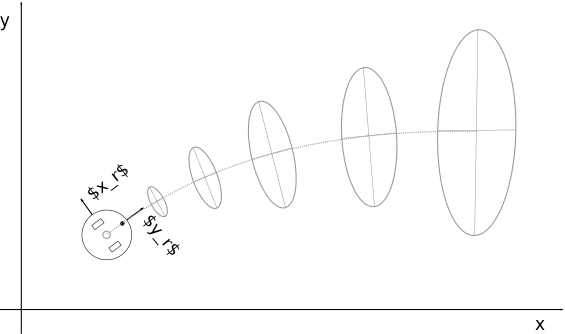
\includegraphics[width=\textwidth]{figs/errorprop_odometry}
	\caption{Two-dimensional Normal distribution depicting growing uncertainty as the robot moves. Albeit starting with equal
    uncertainty in $x$ and $y$, the large effect of small errors in orientation lets the error grow faster in $y$-direction of the robot.}
	\label{fig:errorprop_odometry}
\end{figure}

If only there were a way to correct this unbounded error with some sort of sensor measurement! However, even such sensor measurements would be affected by uncertainty. We'll get back to such a correction shortly (or you can check out Section \ref{sec:KF} if you're really champing at the bit).

Similar to this example, when estimating distance and angle to a line feature from point cloud data, the uncertainty of the random variables describing distance and angle to the line are somewhat related to the uncertainty of \emph{each} point measured on the line. These relationships are formally captured by the \emph{error propagation law}\index{Error Propagation Law}.

The key intuition behind the error propagation law is that the variance of each component that contributes to a random variable should
be weighted as a function of how strongly this component influences this random variable. Measurements that have little effect on the
aggregated random variable should also have little effect on its variance and vice versa. ``How strongly'' one variable affects another
can be expressed by the ratio of how small changes of the first variable relate to small changes in the second one. This is nothing else
than the partial derivative of the first variable with respect to the second. For example, let $y=f(x)$ be a function that maps a random variable $x$, e.g., a sensor reading, to a random variable $y$, e.g., a feature. Let the standard deviation of $x$ be given by $\sigma_x$. We can then calculate the variance $\sigma_y^2$ by
\begin{equation}
\sigma_y^2=\left(\frac{\partial f}{\partial x}\right)^2 \sigma_x^2
\end{equation}
In case $\mathbf{y}=f(\mathbf{x})$ is a multivariable function that maps $n$ inputs to $m$ outputs, variances between these
variables may be represented by \emph{covariance matrices}\index{Covariance Matrix}, a representation of the various combinations in
which these variables may affect one another, one by one. A covariance matrix holds the variance of each variable along its diagonal and is zero otherwise, if the random variables are not correlated. We can then write
\begin{equation}
\Sigma^Y= J \Sigma^X J^T
\end{equation}
where $\Sigma^X$ and $\Sigma^Y$ are the covariance matrices holding the variances of the input and output variables, respectively, and
$J$ is a $m \times n$ \emph{Jacobian} matrix, which holds the partial derivatives $\frac{\partial f_i}{\partial x_j}$. As $J$ has $n$ columns, each row contains partial derivatives with respect to $x_1$ to $x_n$.

\subsection{Example: Line Fitting}\label{sec:linefitting}
Let's consider an example of estimating the angle $\alpha$ and distance $r$ of a line from a set of points given by $(\rho_i,\theta_i)$ using Equations~\ref{eq:linealpha}--\ref{eq:liner}. We can now express the relationship of changes of a variable such as $ \rho_i$ to changes in $ \alpha$ by
\begin{equation}
\frac{\partial \alpha}{\partial \rho_i}
\end{equation}
Similarly, we can calculate $ \frac{\partial \alpha}{\partial \theta_i}$, $ \frac{\partial r}{\partial \rho_i}$ and $ \frac{\partial r}{\partial \theta_i}$. We can actually do this, because we have derived analytical expressions for $ \alpha$ and $ r$ as a function of $ \theta_i$ and $ \rho_i$ in Chapter~\ref{chap:feature_extraction}.

We are now interested in deriving equations for calculating the variance of $ \alpha$ and $ r$ as a function of the variances of the distance measurements. Let's assume each distance measurement $ \rho_i$ has variance $ \sigma^2_{\rho_i}$ and each angular measurement $ \theta_i$ has variance $ \sigma^2_{\theta_i}$. We now want to calculate $ \sigma^2_{\alpha}$ as the weighted sum of  $ \sigma^2_{\rho_i}$ and $ \sigma^2_{\theta_i}$, each weighted by its influence on $ \alpha$.
More generally, if we have $ I$ input variables $ X_i$ and $K$ output variables $Y_k$, the covariance matrix of the output variables $ \sigma_Y$ can be expressed as $\sigma_Y^2=\frac{\partial f}{\partial X}^2 \sigma_X^2$ where $\sigma_X$ is the covariance matrix of input variables and $J$ is a Jacobian matrix of a function $ f$ that calculates $Y$ from $X$ and has the form

\begin{equation}
J=\left[
\begin{array}{ccc}
  \frac{\partial f_1}{\partial X_1} & \ldots & \frac{\partial f_1}{\partial X_I}\\
  \vdots & \ldots & \vdots\\
  \frac{\partial f_K}{\partial X_1} & \ldots & \frac{\partial f_K}{\partial X_I}
 \end{array}
 \right]
\end{equation}

In the line fitting example $ F_X$ would contain the partial derivatives of $ \alpha$ with respect to all $ \rho_i$ ($i$-entries) followed by the partial derivates of $ \alpha$ with respect to all $ \theta_i$ in the first row. In the second row, $ F_X$ would hold the partial derivates of $ r$ with respect to $ \rho_i$ followed by the partial derivates of $ r$ with respect to $ \theta_i$. As there are two output variables, $ \alpha$ and $ r$, and $2I$ input variables (each measurement consists of an angle and distance), $ F_X$ is a 2 $\times$ (2$I$) matrix.

The result is therefore a 2$\times$2 covariance matrix that holds the variances of $ \alpha$ and $ r$ on its diagonal.

\subsection{Example: Odometry}
\screencast{https://www.youtube.com/watch?v=ubg_AAM7Zd8}{errorpropagation}
Whereas the line fitting example demonstrated a many-to-one mapping, odometry requires to calculate the variance that results from multiple sequential measurements.  Error propagation allows us here to not only express the robot's position, but also the variance of this estimate. Our ``laundry list'' for this task looks as follows:
\begin{enumerate}
\item What are the input variables and what are the output variables?
\item What are the functions that calculate output from input?
\item What is the variance of the input variables?
\end{enumerate}

As usual, we describe the robot's position by a tuple $ (x,y,\theta)$. These are the three output variables. We can measure the distance each wheel travels $ \Delta s_r$ and $ \Delta s_l$ based on the encoder ticks and the known wheel radius. These are the two input variables. We can now calculate the change in the robot's position by calculating
\begin{eqnarray}
\Delta x  &=& \Delta s cos(\theta)\\
\Delta y  &=& \Delta s sin(\theta)\\
\Delta \theta &=& \frac{\Delta s_r-\Delta s_l}{b}
\end{eqnarray}
with
\begin{equation}
\Delta s=\frac{\Delta s_r + \Delta s_l}{2}
\end{equation}

The new robot's position is then given by
\begin{equation}
f(x,y,\theta,\Delta s_r, \Delta s_l)=[x,y,\theta]^T + [\Delta x \qquad \Delta y \qquad \Delta \theta]^T
\end{equation}
We thus have now a function that relates our measurements to our output variables. What makes things complicated here is that the output variables are a function of their previous values. Therefore, their variance does not only depend on the variance of the input variables, but also on the previous variance of the output variables. We therefore need to write
\begin{equation}\label{eq:errorpropodom}
\Sigma_{p'}=\nabla_p f \Sigma_p \nabla_p f^T + \nabla_{\Delta_{r,l}}f \Sigma_{\Delta}\nabla_{\Delta_{r,l}}f^T
\end{equation}
The first term is the error propagation from a position $ p=[x,y,\theta]$ to a new position $ p'$. For this we need to calculate the partial derivatives of $ f$ with respect to x, y and $ \theta$. This is a 3x3 matrix
\begin{equation}
\nabla_p f=\left[\frac{\partial f}{\partial x} \quad \frac{\partial f}{\partial y} \quad \frac{\partial f}{\partial \theta}\right]=\left[\begin{array}{ccc}1 & 0 & -\Delta s sin(\theta +\Delta \theta /2)\\0 & 1 & \Delta s cos(\theta + \Delta \theta/2)\\0 & 0 &1\end{array}\right]
\end{equation}
The second term is the error propagation of the actual wheel slip. This requires calculating the partial derivatives of $ f$ with respect to $ \Delta s_r$ and $ \Delta s_l$, which is a 3x2 matrix. The first column contains the partial derivatives of $ x,y,\theta$ with respect to $ \Delta s_r$. The second column contains the partial derivatives of $ x,y,\theta$ with respect to $ \Delta s_l$:
\begin{scriptsize}
\begin{equation}
\nabla_{\Delta_{r,l}} f=\left[
\begin{array}{ccc}
\frac{1}{2}\cos(\theta+\frac{\Delta \theta/2}{b})
-\frac{\Delta s}{2b}\sin(\theta+\frac{\Delta \theta}{b})
& \quad & \frac{1}{2}\cos(\theta+\frac{\Delta \theta/2}{b})
-\frac{\Delta s}{2b}\sin(\theta+\frac{\Delta \theta}{b})
\\
\frac{1}{2}\sin(\theta+\frac{\Delta \theta/2}{b})
+\frac{\Delta s}{2b}\cos(\theta+\frac{\Delta \theta}{b})
& \quad & \frac{1}{2}\sin(\theta+\frac{\Delta \theta/2}{b})
+\frac{\Delta s}{2b}\cos(\theta+\frac{\Delta \theta}{b})
\\
\frac{1}{2} & \quad & -\frac{1}{2}
\end{array}
\right]
\end{equation}
\end{scriptsize}

Finally, we need to define the covariance matrix for the measurement noise. As the error is proportional to the distance traveled, we can define $ \Sigma_{\Delta}$ by
\begin{equation}
\Sigma_{\Delta}=\left[\begin{array}{cc}k_r|\Delta s_r| & 0\\0 & k_l|\Delta s_l|\end{array}\right]
\end{equation}
Here $ k_r$ and $ k_l$ are constants that need to be found experimentally and $ |\cdot |$ indicating the absolute value of the distance traveled. We also assume that the error of the two wheels is independent, which is expressed by the zeros in the matrix.

We now have all ingredients for Equation~\ref{eq:errorpropodom}, allowing us to calculate the covariance matrix of the robot's pose much like shown in Figure~\ref{fig:errorprop_odometry}.

\section{The Kalman Filter}
The location of a robot is subject to uncertainty due to wheel-slip and (to a much lesser extent) encoder noise. We learned in the past how the variance in position can be derived from the variance of the robot's drivetrain using the error propagation law and the forward kinematics of the robot. One can see that this error is continuously increasing unless the robot has additional observations, e.g., some external measurement of motion.
%This update can be formally done using Bayes' rule, which relates the likelihood to be at a certain position given that the robot sees a certain feature to the likelihood to see this feature at the hypothetical location. For example, a robot that drives towards a wall will become less and less certain of its position (action update) until it encounters the wall (perception update).
With these measurements, the robot could then use its sensor model that relates its observation with possible positions.
Its real location would therefore be somewhere between its original belief based on error propagation and where the sensor tells it to be.
%Bayes' rule allows us to perform this location for discrete locations and discrete sensor error distributions. This is inconvenient as we are used to represent our robot's position with a 2D Gaussian distribution. Also, it seems much easier to just change the mean and variances of this Gaussian instead of updating hundreds of variables.
The goals of this section are:

\begin{itemize}
\item to introduce a technique known as the Kalman filter to perform action and perception updates exclusively using Gaussian distributions.
\item to formally introduce the notion of a feature map.
\item to develop an example that puts everything we learned so far together: forward kinematics, error propagation, and sensor noise.
\end{itemize}

\subsection{Optimal Sensor Fusion}
The Kalman filter is an optimal way to fuse observations that follow a Gaussian distribution. The Kalman filter has a prediction step and an update step. The prediction step uses a dynamical model of the system (such as the forward kinematics of your robot) and the update step uses a sensor model (such as the error distribution calibrated from its sensors). The Kalman filter does not only update the state of the system (the robot's position) but also its variance. For this, it requires knowledge of all the variances involved in the system (e.g., wheel-slip and sensor error) and uses them to weigh each measurement accordingly. Before providing the equations for the Kalman filter, we will make use of a simple example that explains what ``optimal'' means in this context.

 Let $ \hat{q_1}$ and $ \hat{q_2}$ be two different estimates of a random variable and $ \sigma^2_1$ and $ \sigma^2_2$ their variances, respectively. Let $ q$ be the true value. This could be the robot's position, e.g. The observations have different variances when they are obtained by  different means, say using odometry for $ \hat{q_1}$ and by using the location of a known feature for $ \hat{q_2}$. We can now define the weighted mean-square error
 \begin{equation}
S=\displaystyle\sum_{i=1}^{n}\frac{1}{\sigma_i} (q-\hat{q_i})^2
\end{equation}
that is, $ S$ is the sum of the errors of each observation $ \hat{q_i}$ weighted by its standard deviation $ \sigma_i$. Each error is weighted  with its standard deviation to put more emphasis on observations whose standard deviation is low. Minimizing  $S$ for $n=2$ yields the following optimal expression for $q$:
\begin{equation}
q=\frac{\hat{q_1}\sigma_2^2}{\sigma_1^2+\sigma_2^2}+\frac{\hat{q_2}\sigma_1^2}{\sigma_1^2+\sigma_2^2}
\end{equation}
or, equivalently,
\begin{equation}
q=\hat{q_1}+\frac{\sigma_1^2}{\sigma_1^2+\sigma_2^2}(\hat{q_2}-\hat{q_1})\label{eq:optimalfusion}
\end{equation}

We have now derived an expression for fusing two observations with different errors that provably minimizes the error between our estimate and the real value. As $q$ is a linear combination of two random variables (Section~\ref{sec:lcombrandom}, the new variance is given by
\begin{equation}
\sigma^2=\frac{1}{\frac{1}{\sigma_1^2}+\frac{1}{\sigma_2^2}}
\end{equation}
Interestingly, the resulting variance is smaller than both $\sigma_1$ and $\sigma_2$, that is, adding additional observation always helps  reducing accuracy instead of introducing more uncertainty.

\subsection{Integrating prediction and update: The Kalman Filter}
Although we have introduced the problem above as fusing two observations of the same quantity and weighting them by their variance, we can also interpret the equation above as an update step that calculates a new estimate of an observation based on its old estimate and a measurement. Remember step (4) from above: $ \hat{q_2}-\hat{q_1}$ is nothing else then the difference between what the robot actually sees and what it thinks it should see. This term is known as innovation in Kalman lingo. We can now
rewrite (\ref{eq:optimalfusion}) from above into
\begin{equation}
\hat{x}_{k+1}=\hat{x}_k+K_{k+1}\tilde{y}_{k+1}
\end{equation}
Here, $ \hat{x}_k$ is the state we are interested in at time $ k$, $ K_{k+1}=\frac{\sigma_1^2}{\sigma_1^2+\sigma_2^2}$ the Kalman gain, and $ \tilde{y}_{k+1}=\hat{q_2}-\hat{q_1}$  the innovation. Unfortunately, there are few systems that allow us to directly measure the information we are interested in. Rather, we obtain a sensor measurement $ z_k$ that we need to convert into our state somehow. You can think about this the other way too and predict your measurement $ z_k$ from your state $ x_k$. This is done using the observation model $ H_k$, so that
\begin{equation}
\tilde{y}_{k}=z_k-H_k x_k
\end{equation}
In our example $ H_k$ was just the identity matrix; in a robot position estimation problem $ H_k$ is a function that would predict how a robot would observe a shift in position through a sensor. As you can see, all the weighting based on variances is done in the Kalman gain $ K$.
The perception update step shown above only half of what the Kalman filter does. The first step is the prediction step, which corresponds to the action we already know. In fact, the variance update in the Kalman filter is exactly the same as we learned during error propagation. Before going into any more details on the Kalman filter, it is time for a brief disclaimer: the Kalman filter only works for linear systems. Forward kinematics of even the simplest robots are mostly intrinsically non-linear, and so are observation models that relate sensor observations and the robot position. Non-linear systems can be dealt with the Extended Kalman Filter, which linearizes both the process model and sensor model around the current state.

\section{Extended Kalman Filter}\label{sec:EKF}
In the extended Kalman filter, the state transition and observation models do not need to be linear functions of the state but may instead be differentiable functions. The action prediction step looks as follows:
\begin{equation}
\hat{\boldsymbol{x}}_{k'|k-1} = f(\hat{\boldsymbol{x}}_{k-1|k-1}, \boldsymbol{u}_{k-1})
\end{equation}
Here $ f()$ is a function of the old state $ \boldsymbol{x}_{k-1}$ and control input $ \boldsymbol{u}_{k-1}$. This is nothing else as the odometry update we are used to, where $ f()$ is a function describing the forward kinematics of the robot, $ \boldsymbol{x}_k$ its position and $ \boldsymbol{u}_k$ the wheel-speed we set.

We can also calculate the covariance matrix of the robot position

\begin{equation}
\boldsymbol{P}_{k'|k-1} = \nabla_{x,y,\theta}f \boldsymbol{P}_{k-1|k-1}\nabla_{x,y,\theta}f^T + \nabla_{\Delta_{r,l}}f\boldsymbol{Q}_{k-1}\nabla_{\Delta_{r,l}}f
\end{equation}

This is nothing else as the error propagation law applied to the odometry of the robot with $ \boldsymbol{Q}_k$ the covariance matrix of the wheel-slip and the Jacobian matrices of the forward kinematic equations $ f()$ with respect to the robot's position (indicated by the index $ x,y,\theta$) and with respect to the wheel-slip of the left and right wheel.

The perception update step looks as follows:

\begin{eqnarray}
\hat{\boldsymbol{x}}_{k|k'} &=& \hat{\boldsymbol{x}}_{k'|k-1} + \boldsymbol{K}_{k'}\tilde{\boldsymbol{y}}_{k'}\\
\boldsymbol{P}_{k|k'} &=& (I - \boldsymbol{K}_{k'} {\boldsymbol{H}_{k'}}) \boldsymbol{P}_{k'|k-1}
\end{eqnarray}

At this point the indices $ k$ should start making sense. We are calculating everything twice: once we update from $ k-1$ to an intermediate result $ k'$ during the action update, and obtain the final result after the perception update where we go from $ k'$ to $ k$.

We need to calculate three additional variables:
\begin{enumerate}
\item The innovation $ \tilde{\boldsymbol{y}}_{k}=\boldsymbol{z}_{k}-h(\hat{\boldsymbol{x}}_{k|k-1})$
\item The covariance of the innovation $\boldsymbol{S}_{k}={\boldsymbol{H}_{k}}\boldsymbol{P}_{k|k-1}{\boldsymbol{H}_{k}^\top}+\boldsymbol{R}_{k}$
\item The (near-optimal)  Kalman gain $ \boldsymbol{K}_{k}=\boldsymbol{P}_{k|k-1}{\boldsymbol{H}_{k}^\top}\boldsymbol{S}_{k}^{-1}$
\end{enumerate}
Here $ h()$ is the observation model and $ \boldsymbol{H}$ its Jacobian. How these equations are derived is involved (and is one of the fundamental results in control theory), but the idea is the same as introduced above: we wish to minimize the error of the prediction.

\subsection{Odometry using the Kalman Filter}
We will show how a mobile robot equipped with a laser scanner can correct its position estimate by relying on unreliable odometry, unreliable sensing, but a correct map, in an optimal way.
Whereas the update step is equivalent to forward kinematics and error propagation we have seen before, the observation model and the ``innovation'' require additional steps to perform odometry.

\paragraph{1. Prediction}
We assume for now that the reader is familiar with calculating $ \hat{\boldsymbol{x}}_{k'|k-1}=f(x,y,\theta)^T$ and its variance $ \boldsymbol{P}_{k'|k-1}$. Here, $ \boldsymbol{Q}_{k-1}$, the covariance matrix of the wheel-slip error,  is given by
\begin{equation}
\boldsymbol{Q}_{k-1}=\left[\begin{array}{cc}k_r|\Delta s_r & 0\\0 & k_l|\Delta s_l|\end{array}\right]
\end{equation}
where $ \Delta s$ is the wheel movement of the left and right wheel and $ k$ are constants. See also the odometry lab for detailed derivations of these calculations and how to estimate $ k_r$ and $ k_l$.  The state vector $ \boldsymbol{\hat{x}_{k'|k-1}}$ is a 3$\times$1 vector, the covariance matrix $ \boldsymbol{P_{k'|k-1}}$ is a 3$\times$3 matrix, and $ \nabla_{\Delta_{r,l}}$ that is used during error propagation is a 3$\times$ matrix. See the error propagation section for details on how to calculate $ \nabla_{\Delta_{r,l}}$.

\textbf{TODO: EDIT THIS FROM MAPPING TO LOCALIZATION ONLY}
\paragraph{2. Observation}
Let us now assume that we can detect the motion of the robot through an optical flow sensor \textbf{TODO.}
%\paragraph{2. Observation}
%Let us now assume that we can detect line features $ \boldsymbol{z}_{k,i}=(\alpha_i,r_i)^T$, where $ \alpha$ and $ r$ are the angle and distance of the line from the coordinate system of the robot. These line features are subject to variances $ \sigma_{\alpha,i}$ and $ \sigma_{r,i}$, which make up the diagonal of $ \boldsymbol{R}_{k}$. See the line detection section for a derivation of how angle and distance as well as their variance can be calculated from a laser scanner. The observation is a 2x1 matrix.

\paragraph{3. Measurement Update}
%We assume that we can uniquely identify the lines we are seeing and retrieve their real position from a map. This is much easier for unique features, but can be done also for lines by assuming that our error is small enough and we therefore can search through our map and pick the closest lines. As features are stored in global coordinates, we need to transpose them into how the robot would see them. In practice this is nothing but a list of lines, each with an angle and a distance, but this time with respect to the origin of the global coordinate system. Transposing them into robot coordinates is straightforward. With  $ \hat{\boldsymbol{x}}_{k}=(x_{k},y_{k},\theta_k)^T$ and $ m_i=(\alpha_i,r_i)$ the corresponding entry from the map, we can write

\begin{equation} h(\hat{\boldsymbol{x}}_{k|k-1})=\left[\begin{array}{c}\alpha_{k,i}\\r_{k,i}\end{array}\right]=h(\boldsymbol{x},m_i)=\left[\begin{array}{c}\alpha_i-\theta\\r_i-(x cos(\alpha_i)+y sin(\alpha_i)\end{array}\right]
\end{equation}

%and calculate its Jacobian $ \boldsymbol{H}_{k}$ as the partial derivatives of $ \alpha$ to $ x,y,\theta$ in the first row, and the partial derivatives of $ r$ in the second. How to calculate $ h()$ to predict the radius at which the robot should see the feature with radius $ r_i$ from the map is illustrated in the figure below.


%\begin{mdframed}
%Example on how to predict the distance to a feature the robot would see given its estimated position and its known location from a map.
%\end{mdframed}

\paragraph{4. Matching}
%We are now equipped with a measurement $ \boldsymbol{z}_k$ and a prediction $ h(\hat{\boldsymbol{x}}_{k|k-1})$ based on all features stored in our map. We can now calculate the innovation
\begin{equation}
\tilde{\boldsymbol{y}}_{k}=\boldsymbol{z}_{k}-h(\hat{\boldsymbol{x}}_{k|k-1})
\end{equation}

%which is simply the difference between each feature that we can see and those that we predict from the map. The innovation is again a 2x1 matrix.

\paragraph{5. Estimation}
We now have all the ingredients to perform the perception update step of the Kalman filter:

\begin{eqnarray}
\hat{\boldsymbol{x}}_{k|k'} &=& \hat{\boldsymbol{x}}_{k'|k-1} + \boldsymbol{K}_{k'}\tilde{\boldsymbol{y}}_{k'}\\
\boldsymbol{P}_{k|k'} &=& (I - \boldsymbol{K}_{k'} {\boldsymbol{H}_{k'}}) \boldsymbol{P}_{k'|k-1}
\end{eqnarray}

%It will provide us with an update of our position that fuses our odometry input and information  that we can extract from features in the environment in a way that takes into account their variances. That is, if the variance of your previous position is high (because you have no idea where you are), but the variance of your measurement is low (maybe from a GPS or a symbol on the Ratslife wall), the Kalman filter will put more emphasis on your sensor. If your sensors are poor (maybe because you cannot tell different lines/walls apart), more emphasis will be on the odometry.

%As the state vector is a 3x1 vector and the innovation a 2x1 matrix, the Kalman gain must be a 3x2 matrix. This can also be seen when looking at the covariance matrix that must come out as a 3x3 matrix, and knowing that the Jacobian of the observation function is a 2x3 matrix. We can now calculate the covariance of the innovation and the Kalman gain using

\begin{eqnarray}
\boldsymbol{S}_{k}&=&{\boldsymbol{H}_{k}}\boldsymbol{P}_{k|k-1}{\boldsymbol{H}_{k}^\top}+\boldsymbol{R}_{k}\\
\boldsymbol{K}_{k}&=&\boldsymbol{P}_{k|k-1}{\boldsymbol{H}_{k}^\top}\boldsymbol{S}_{k}^{-1}
\end{eqnarray}

\section{Take-home lessons}
\begin{itemize}
\item Uncertainty can be expressed by means of a probability density function.
\item More often than not, the Gaussian distribution is chosen as it allows treating error with powerful analytical tools.
\item In order to calculate the uncertainty of a variable that is derived from a series of measurements, we need to calculate a weighted sum in which each measurement's variance is weighted by its impact on the output variable. This impact is expressed by the partial derivative of the function relating input to output.
\end{itemize}

\section*{Exercises}\small
\begin{enumerate}
\item Given two observations $\hat{q}_1$ and $\hat{q}_2$ with variances $\sigma_1$ and $\sigma_2$ of a normal distributed process with actual value $\hat{q}$, an optimal estimate can be calculated by minimizing the expression
\begin{equation}
\nonumber
S=\frac{1}{\sigma_1^2}(\hat{q}-\hat{q}_1)^2+\frac{1}{\sigma_2^2}(\hat{q}-\hat{q}_2)^2
\end{equation}
Calculate $\hat{q}$ so that $S$ is minimized.
\item An ultrasound sensor measures distance $x=c\Delta t/2$. Here, $c$ is the speed of sound and $\Delta t$ is the difference in time between emitting and receiving a signal.
\begin{enumerate}
\item Let the variance of your time measurement $\Delta t$ be $\sigma_t^2$. What can you say about the variance of $x$, when $c$ is assumed to be constant? Hint: how does a change in $\Delta t$ affect $x$?
\item Now assume that $c$ is changing depending on location, weather, etc.\ and can be estimated with variance $\sigma_c^2$. What is the variance of $x$ now?
\end{enumerate}
\item Consider a unicycle that turns with angular velocity $\dot{\phi}$ and has radius $r$. Its speed is thus a function of $\dot{\phi}$ and $r$ and is given by
\begin{equation}
\nonumber
v=f(\dot{\phi},r)=r\dot{\phi}
\end{equation}
Assume that your measurement of $\dot{\phi}$ is noisy and has a standard deviation $\sigma_{\dot{\phi}}$.  Use the error propagation law to calculate the resulting variance of your speed estimate $\sigma_v^2$.
\item Consider a scenario in which a robot can localize itself against landmarks. Describe what happens to the robot's positional error in the following three cases:
\begin{enumerate}
\item the landmark location is known and the robot can reliably localize to it,
\item the landmark location has a variance and the robot can realibly localize to it,
\item both the landmark and localization mechanism have a variance.
\end{enumerate}
\item Write a program that graphically illustrate merging observations with two different variances in 1D and 2D.
\end{enumerate}
\normalsize
